\section{Model confidence sets: retained main comparison}\label{sup:v13-mcs}

Joint comparison leaves matched historical methods alongside alternatives in most sets, with a single historical method surviving in only a small minority. These results support retaining historical controls while leaving many alternatives uneliminated under the fixed bootstrap approximation. Non-elimination does not establish equal predictive risk. Table~\ref{tab:v10-mcs-main} reports surviving methods, with identical observed-loss patterns explained separately in Supplement Section S31. Supplement Section S31 retains every set, method p-value, equivalence class and prior unavailable method.

These confidence sets use the original comparison inventory; the later validation rules are reported separately in Section~\ref{sup:v13-checks}.

\begin{table}[!htbp]\centering\footnotesize
\setlength{\tabcolsep}{4pt}
\caption{Ninety-percent model confidence sets across all planned comparisons. Counts retain their comparison or conditional-procedure denominators.}\label{tab:v10-mcs-main}
\begin{tabular}{lrrrrr}\toprule
Group & Complete & Matched history & Sole historical & Conditional & Unavailable \\
 & / planned & included & method & excluded & procedures \\ \midrule
FX original & 4/4 & \makebox[3.2em][r]{2/4} (\makebox[2.9em][r]{50.0}\%) & \makebox[3.2em][r]{0/4} (\makebox[2.9em][r]{0.0}\%) & \makebox[3.2em][r]{39/66} (\makebox[2.9em][r]{59.1}\%) & 6 \\
FX earlier period & 4/4 & \makebox[3.2em][r]{3/4} (\makebox[2.9em][r]{75.0}\%) & \makebox[3.2em][r]{0/4} (\makebox[2.9em][r]{0.0}\%) & \makebox[3.2em][r]{1/15} (\makebox[2.9em][r]{6.7}\%) & 2 \\
Treasury bills & 4/4 & \makebox[3.2em][r]{4/4} (\makebox[2.9em][r]{100.0}\%) & \makebox[3.2em][r]{0/4} (\makebox[2.9em][r]{0.0}\%) & \makebox[3.2em][r]{11/74} (\makebox[2.9em][r]{14.9}\%) & 4 \\
Other NYFed panels & 48/48 & \makebox[3.2em][r]{46/48} (\makebox[2.9em][r]{95.8}\%) & \makebox[3.2em][r]{0/48} (\makebox[2.9em][r]{0.0}\%) & \makebox[3.2em][r]{110/384} (\makebox[2.9em][r]{28.6}\%) & 48 \\
Same-record daily FX & 4/4 & \makebox[3.2em][r]{4/4} (\makebox[2.9em][r]{100.0}\%) & \makebox[3.2em][r]{2/4} (\makebox[2.9em][r]{50.0}\%) & \makebox[3.2em][r]{5/8} (\makebox[2.9em][r]{62.5}\%) & 0 \\
CFTC & 34/34 & \makebox[3.2em][r]{31/34} (\makebox[2.9em][r]{91.2}\%) & \makebox[3.2em][r]{0/34} (\makebox[2.9em][r]{0.0}\%) & \makebox[3.2em][r]{31/136} (\makebox[2.9em][r]{22.8}\%) & 0 \\
All comparisons & 98/98 & \makebox[3.2em][r]{90/98} (\makebox[2.9em][r]{91.8}\%) & \makebox[3.2em][r]{2/98} (\makebox[2.9em][r]{2.0}\%) & \makebox[3.2em][r]{197/683} (\makebox[2.9em][r]{28.8}\%) & 60 \\
\bottomrule\end{tabular}
\par\smallskip\begin{minipage}{.98\linewidth}\footnotesize
Matched history includes corrected and ordinary empirical headroom reports, excluding rolling references and nearest-neighbor baselines; conditional exclusions count complete procedures.
Identical losses can leave several methods tied, so the sole-method column counts only sets containing exactly one historical procedure.
The \href{https://github.com/ByronLi0207/financial-mathematics-paper-20261020/blob/submission-final/EXTENDED_RESULTS.md#asmbi-extended-s31}{extended confidence-set results} retain all tied loss patterns, secondary membership counts and unavailable procedures; related comparisons are not independent replications.
\end{minipage}\end{table}


\FloatBarrier
\section{Validation extensions and a retrospective decision rule}\label{sup:v13-checks}

\paragraph{Post-failure solver check.}
The solver change designed after the failure was not adopted. Only 6 of 10 previously converged fits reproduced forecasts within $10^{-6}$ pointwise relative error. Residual and duality-gap thresholds were not relaxed. The pre-specified gate therefore prevented all three failed 99\% comparisons from running with this change. Their original unavailable values remain, leaving both aggregate tail-level conditions undetermined. The \href{https://github.com/ByronLi0207/financial-mathematics-paper-20261020/tree/revision-v13/results/v13/tau-repair}{complete numerical check} retains every agreement failure and unrun comparison.

\paragraph{Longer validation in the New York Fed series.}
Across-series median loss falls under longer validation at both horizons, extending the direction found in CFTC. Table~\ref{tab:v13-validation} reports both regression variants, including the failed short-horizon median-improvement condition for the four-feature variant. Figure~\ref{fig:v13-validation} retains every sequence beside the CFTC comparisons rather than pooling their evidence.

\begin{table}[!htbp]\centering\footnotesize\setlength{\tabcolsep}{3pt}
\caption{New York Fed validation-length comparisons on the unchanged evaluation sample. Entries are across-series median excess loss relative to corrected historical headroom, with changes in percentage points and selections of the ordinary empirical limit. Every method/horizon row contains all thirteen series.}\label{tab:v13-validation}
\begin{tabular}{lrrrrlll}\toprule
Method & $H$ & 52 weeks (\%) & 156 weeks (\%) & Change (pp) & $\infty$: 52/156 & Median screen & Shrinkage screen\\\midrule
Full regression & 6 & +6.68 & -1.13 & -7.81 & 6 / 9 & Pass & Pass \\
Full regression & 24 & +40.47 & +5.02 & -35.45 & 3 / 9 & Pass & Pass \\
Four-feature & 6 & +3.26 & -0.95 & -4.22 & 5 / 7 & Fail & Pass \\
Four-feature & 24 & +24.88 & +6.21 & -18.67 & 4 / 9 & Pass & Pass \\
\bottomrule\end{tabular}
\par\smallskip\begin{minipage}{.98\linewidth}\footnotesize The two screens are the pre-specified across-series median-improvement and increased infinite-penalty-selection conditions. Arm-median changes are not medians of paired series changes.\end{minipage}
\end{table}

The original validation origins are 329--380; longer validation uses 243--398 at the short horizon and 225--380 at the longer horizon. Evaluation remains 405--681, with 277 issues. Thus the short-horizon endpoint also advances eighteen weeks and changes the validation refit phase; this is not a causal length-only comparison. The longer-horizon endpoint is unchanged. Differences between arm medians also need not describe a typical series: for full regression, the paired-change median is +0.00 and -44.10 percentage points, respectively. All source, candidate and failure records remain in the \href{https://github.com/ByronLi0207/financial-mathematics-paper-20261020/tree/revision-v13/results/v13/nyfed-validation}{complete validation-length results}; related weekly categories are not independent dealer replications.

\begin{figure}[!htbp]\centering
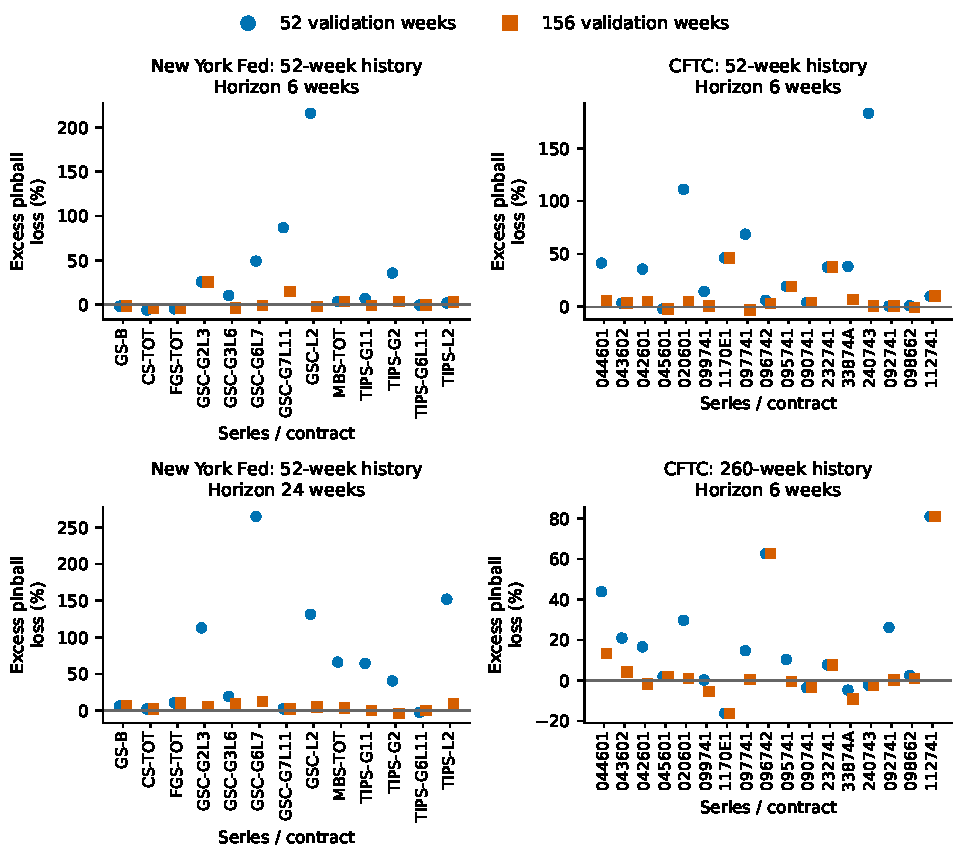
\includegraphics[width=.98\linewidth]{figures/v13-validation-length.pdf}
\caption{Full-regression losses under short and long validation samples, with each reporting system retaining its own sources and histories. Points use unchanged evaluation origins; positive excess means higher loss than matched corrected historical headroom. The New York Fed short-horizon extension also changes the endpoint and refit phase; shortened source labels omit the common PDPOS prefix, so GS-B means PDPOSGS-B.}\label{fig:v13-validation}
\end{figure}

\FloatBarrier
\paragraph{The retrospective validation protocol.}
The rule uses the six-point penalty menu, longer validation, and a historical default. Weekly validation contains 156 issues and FX validation contains 5,760; regression replaces corrected historical headroom only when its validation advantage exceeds one paired HAC standard error. Selection and the gate share validation data, and the decision stays fixed over the evaluation segment. Infinite shrinkage gives ordinary empirical headroom, so it must pass the same gate to replace the corrected-rank reference. These settings combine existing forecasting and validation methods without a nominal protection guarantee.

All 62 planned comparisons complete, including 60 weekly cells and both FX periods. The weekly median moves from +14.63\% for ordinary regression with the six-point menu to 0.00\% for the protocol. However, 8 of 60 weekly cells exceed the historical loss by more than 10\%, and the worst excess is +80.98\%. The median condition therefore passes while the tail condition fails. The protocol returns to history in 32 weekly cells and uses regression in 28, as Table~\ref{tab:v13-routing} shows. The adverse cells comprise 7 CFTC comparisons and 1 New York Fed comparison. Both FX periods retain their ordinary-regression gains, 14.77\% and 16.62\%, meeting the gain-retention condition.

\begin{table}[!htbp]\centering\footnotesize\setlength{\tabcolsep}{4pt}
\caption{Historical fallback and adverse outcomes by source, horizon and training history. Counts use every planned comparison in each row; the last column counts protocol excess loss above ten percent.}\label{tab:v13-routing}
\begin{tabular}{lrrr rr}\toprule
Source / period & $H$ & $W$ & Historical fallback & Median excess (\%) & Adverse count\\\midrule
Treasury bills & 6 & 52 & 1 / 1 & +0.00 & 0 \\
Other NY Fed series & 6 & 52 & 8 / 12 & +0.00 & 1 \\
Treasury bills & 24 & 52 & 1 / 1 & +0.00 & 0 \\
Other NY Fed series & 24 & 52 & 10 / 12 & +0.00 & 0 \\
CFTC & 6 & 52 & 6 / 17 & +0.00 & 4 \\
CFTC & 6 & 260 & 6 / 17 & +0.00 & 3 \\
FX, original & 6 & 2880 & 0 / 1 & -14.77 & 0 \\
FX, earlier & 6 & 2880 & 0 / 1 & -16.62 & 0 \\
\bottomrule\end{tabular}
\end{table}

The adverse CFTC cells are 1170E1, 095741, 232741 and 112741 at the shorter history, and 044601, 096742 and 112741 at the longer history. The remaining cell is the New York Fed two-to-three-year Treasury coupon category at the short horizon. The \href{https://github.com/ByronLi0207/financial-mathematics-paper-20261020/tree/revision-v13/results/v13/recommended-protocol}{complete protocol results} retain every comparison, selected penalty, paired gate and fallback route. The protocol was designed after inspecting earlier results, including these evaluation periods, so this is a retrospective test rather than prospective protection evidence.
